\chapter{Discussão e Resultados: Chu-liu/Edmonds vs. Frank}


Wittgenstein, em suas investigações filosóficas, propôs a ideia de ``semelhança de família'' que diz que coisas que pertencem ao mesmo grupo não compartilham necessariamente uma característica definidora, mas sim uma série de características que se sobrepõem de maneiras variadas. Assim, membros de uma ``família'' podem ser semelhantes em alguns aspectos, mas diferentes em outros, criando uma rede complexa de relações.


Chu–Liu/Edmonds e Frank são parentes próximos: perseguem o mesmo objetivo com blocos operacionais semelhantes, mas organizam o enredo de modos distintos — um com voz combinatória, o outro com abordagem primal–dual.


Em linhas gerais, os dois métodos são equivalentes quanto ao resultado (ambos devolvem uma r-arborescência de custo mínimo), mas organizam a mecânica de normalizar → contrair → expandir de maneiras distintas:


O algoritmo de Chu–Liu/Edmonds \cite{chu1965,edmonds1967optimum} é o método clássico para encontrar uma arborescência de custo mínimo em um digrafo com pesos arbitrários. Ele funciona recursivamente, escolhendo a melhor entrada para cada vértice, detectando ciclos e contraindo-os, ajustando os custos conforme necessário. O processo se repete até que não haja mais ciclos, momento em que a arborescência é extraída.


Já o método de Frank \cite{frank1981,frank2014} adota uma abordagem primal–dual, elevando potenciais para criar um subgrafo de arcos de custo reduzido zero e, em seguida, extraindo a arborescência apenas com esses arcos. Ciclos são tratados por contração/expansão, mas sem novos ajustes de custos após a fase inicial.


As principais diferenças e semelhanças entre os dois métodos podem ser resumidas assim:

\begin{itemize}\setlength{\itemsep}{2pt}
    \item \textbf{Paradigma e estrutura:} \emph{Chu–Liu/Edmonds} é apresentado de forma mais \emph{primal/combinatória}: escolhe para cada \(v\neq r\) a sua melhor entrada, forma \(F^*\), e trata ciclos imediatamente por contração com ajuste de custos, repetindo até não haver ciclos.
          \emph{Frank} explicita a visão \emph{primal–dual} em \textbf{duas fases}: (I) elevar potenciais para induzir o subgrafo de zeros \(D_0\) com ao menos uma entrada por vértice (apenas ajustes duais e eventuais contrações de ciclos de arcos apertados), e (II) extrair uma arborescência usando \emph{só} arcos apertados, tratando ciclos por contração/expansão, \textbf{sem} novas alterações de potenciais \cite{frank1981,frank2014,schrijver2003comb}.

    \item \textbf{Papel dos potenciais:} Em \emph{Chu–Liu/Edmonds}, a “normalização” por vértice pode ser vista como potenciais \emph{implícitos} (subtrair mínimos de entradas), atualizados conforme a contração progride. Em \emph{Frank}, os potenciais \(\tilde y\) (ou o dual por cortes laminares) são entidades \emph{explícitas} que guiam a criação de arcos apertados e mantêm \(c'\ge 0\); a laminaridade é parte da prova e da organização da fase I.

    \item \textbf{Estratégia de extração:} \emph{Chu–Liu/Edmonds} extrai a arborescência ao final do processo, enquanto \emph{Frank} a obtém diretamente do subgrafo de zeros \(D_0\) na fase II.

    \item \textbf{Tratamento de ciclos:} \emph{Chu–Liu/Edmonds} intercala extração e contração: assim que \(F^*\) tem um ciclo, contrai e ajusta custos, voltando ao mesmo fluxo. \emph{Frank} contrai apenas ciclos de arcos de custo reduzido zero durante a fase I (quando aparecem) e, na fase II, contrai ciclos surgidos da seleção \emph{sem} mexer nos potenciais, reexpandindo ao final com a remoção de uma única aresta interna do ciclo.

    \item \textbf{Foco na estrutura dual:} \emph{Frank} enfatiza a relação primal–dual, com a família laminar de cortes ativos e a condição de complementaridade primal–dual como pilares centrais. \emph{Chu–Liu/Edmonds} é mais direto, focando na construção combinatória da arborescência.

    \item \textbf{Invariantes e corretude:} \emph{Chu–Liu/Edmonds} tradicionalmente é provado por argumentos combinatórios de custo e correção sob contrações. \emph{Frank} ancora a prova em \textbf{complementaridade primal–dual}: ao final, todas as arestas escolhidas são \emph{apertadas} (\(c'=0\)) e cada corte ativo da família laminar é atravessado exatamente uma vez, igualando valores primal e dual.

    \item \textbf{Extração final:} Em \emph{Chu–Liu/Edmonds}, a seleção “uma entrada por vértice” e a resolução de ciclos acontecem iterativamente durante todo o processo. Em \emph{Frank}, a seleção acontece de uma vez sobre o subgrafo de zeros \(D_0\) produzido na fase I, o que simplifica a justificativa de otimalidade por manter todas as escolhas \emph{apertadas}.

    \item \textbf{Complexidade e implementações:} Ambas as abordagens, em versão direta, rodam em \(O(mn)\); com estruturas adequadas, alcançam \(O(m\log n)\) em variantes conhecidas. A formulação dual explícita de \emph{Frank} facilita raciocinar sobre \emph{cortes apertados}, laminaridade e otimizações guiadas pelo dual.

    \item \textbf{Resumo prático:} Pense em \emph{Chu–Liu/Edmonds} como o roteiro combinatório clássico “escolhe mínimos → contrai ciclo → ajusta e repete”. O método de \emph{Frank} reembala a mesma mecânica sob uma ótica \emph{primal–dual}: primeiro “zeramos” as entradas com potenciais até obter \(D_0\), depois extraímos a arborescência apenas com arcos apertados — e é exatamente essa apertude que certifica a otimalidade.
\end{itemize}


Ambos os métodos são amplamente aplicáveis, e a escolha entre eles pode depender do contexto, da familiaridade com técnicas primal–dual ou combinatórias, e das necessidades específicas de implementação.


Estabelecidos os fundamentos teóricos e as distinções conceituais, uma questão natural emerge: \emph{como essas diferenças se manifestam na prática?} Ambas as abordagens garantem otimalidade, mas será que apresentam desempenhos similares em instâncias reais? A organização primal–dual de Frank, com suas duas fases distintas, oferece vantagens computacionais ou apenas elegância teórica?


Para responder a essas perguntas de forma empírica, realizamos uma bateria de testes sistemáticos comparando as implementações de Chu–Liu/Edmonds e Frank (em suas variantes com e sem heap) em grafos de diferentes tamanhos e densidades. Os objetivos são múltiplos: validar a corretude das implementações, caracterizar o comportamento temporal de cada método, e verificar se as previsões teóricas (como a dominância da Fase I em Frank) se confirmam na prática.

\section{Testes e Resultados}

Para validar a eficácia dos algoritmos de \emph{Chu–Liu/Edmonds} e \emph{Frank}, realizamos uma série de testes em diferentes instâncias de grafos direcionados. Os testes foram projetados para avaliar não apenas a correção dos algoritmos, mas também seu desempenho em termos de tempo de execução e uso de memória.

\subsection{Metodologia}

Geramos digrafos enraizados aleatórios com \(|V|\in[100,200]\) e \(|A|\in[n,3n]\), pesos inteiros uniformes em \([1,20]\), e conectividade a partir da raiz \(r0\) garantida por uma construção incremental. Em cada instância (arquivo \texttt{tests.py}):
\begin{itemize}\setlength{\itemsep}{1pt}
    \item removemos arestas que entram em \(r0\) (normalização compatível com as formulações);
    \item executamos \emph{Chu–Liu/Edmonds} e as duas variantes da Fase II de \emph{Frank} (versão direta e com heap) sobre o subgrafo de zeros produzido na Fase I;
    \item comparamos os custos retornados e verificamos a \emph{condição dual} (complementaridade) para ambas as soluções de Frank;
    \item registramos resultado e tempo total por instância em CSV.
\end{itemize}

\subsection{Resultados}

Nas instâncias geradas, os três construtores de arborescência retornam sempre o mesmo custo, e as duas verificações da condição de complementaridade (dual) passam em 100\% dos casos reportados no CSV. Isso corrobora a corretude das implementações e a equivalência entre \emph{Chu--Liu/Edmonds} e \emph{Frank} no valor ótimo (cf. Seções anteriores e \cite{frank2014,schrijver2003comb}).

Do ponto de vista de desempenho, a decomposição temporal por etapas evidencia três fatos principais:
\begin{itemize}\setlength{\itemsep}{2pt}
    \item A Fase~I (normalização primal--dual/elevação de potenciais) domina o tempo total para os tamanhos \(|V|\in[100,200]\) e \(|A|\in[n,3n]|\): tipicamente responde pela maior parcela do tempo por instância, ao passo que o tempo de \emph{Chu--Liu/Edmonds} é menor e as Fases~II são uma fração residual.
    \item Entre as duas variantes de Fase~II, a versão com heap (v2) é sistematicamente mais rápida que a versão direta (v1). Observamos ganhos mediana/mediana na ordem de\;3--8\,$\times$ (histograma de speedup), compatíveis com a troca de uma varredura sequencial por extrações de menor prioridade em \(O(\log n)\).
    \item As estatísticas estruturais do \emph{Chu--Liu/Edmonds} mostram número de contrações e profundidade de recursão pequenos na maioria dos casos (tipicamente 0--3), com alguns outliers; isso é consistente com o limite \(O(n)\) para o número de contrações \cite{schrijver2003comb}. O tamanho do subgrafo de zeros \(D_0\) cresce aproximadamente linearmente com \(|V|\), como esperado pelo critério de “uma entrada apertada por vértice”. O pico de memória observado na Fase~I ficou bem abaixo de 1\,MB nas instâncias testadas.
\end{itemize}

As Figuras~\ref{fig:times-boxplot}--\ref{fig:d0-vs-v} resumem esses achados. O boxplot (Fig.~\ref{fig:times-boxplot}) mostra a distribuição dos tempos de cada etapa; nota-se que a Fase~I concentra a maior variabilidade e mediana mais alta. A nuvem tempo~vs.~\(|A|\) (Fig.~\ref{fig:time-vs-edges}) indica crescimento aproximadamente linear nas faixas testadas. O histograma de speedup (Fig.~\ref{fig:speedup}) evidencia vantagem consistente da variante com heap na Fase~II. Por fim, as distribuições de contrações/profundidade (Fig.~\ref{fig:contr-depth}) e de pico de memória (Fig.~\ref{fig:peakmem}) são concentradas em valores baixos, enquanto o gráfico \(|A(D_0)|\)~vs.~\(|V|\) (Fig.~\ref{fig:d0-vs-v}) sugere proporcionalidade entre o tamanho de \(D_0\) e o número de vértices.

\begin{figure}[H]
    \centering
    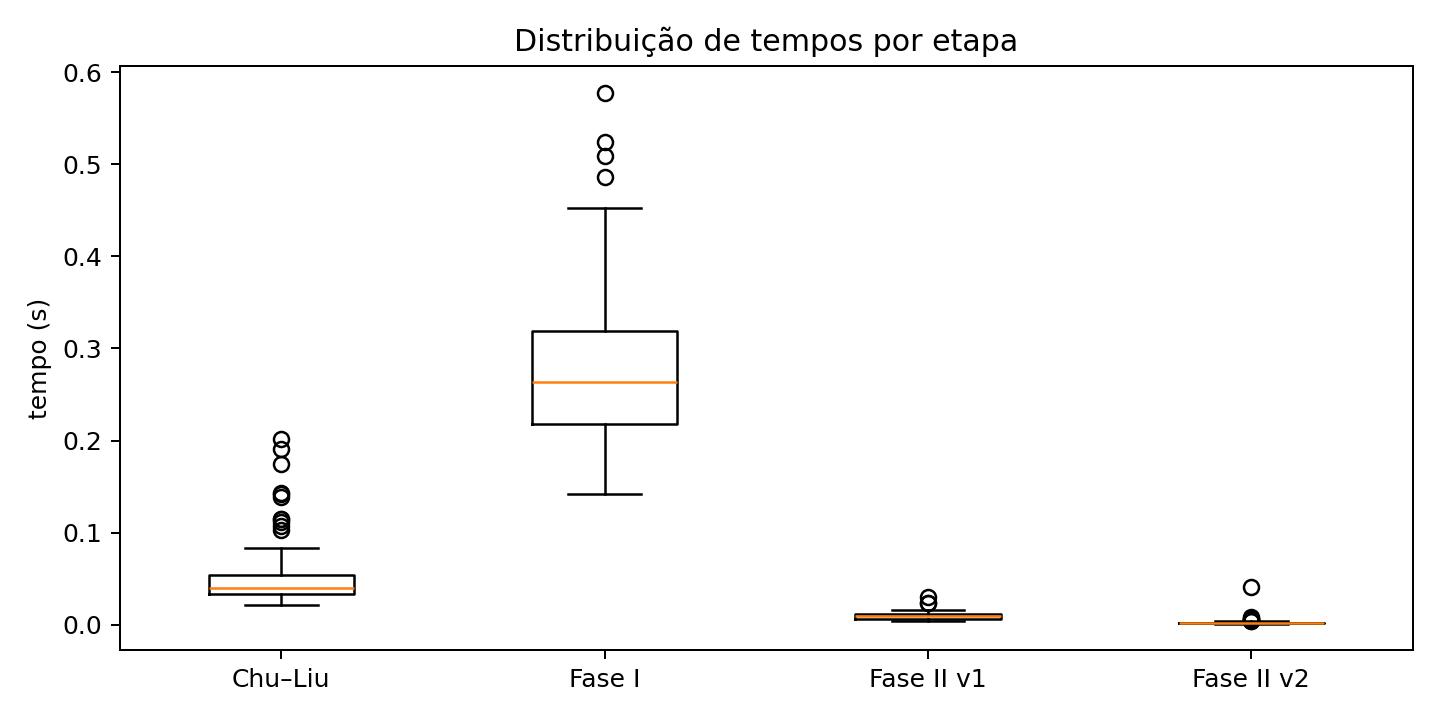
\includegraphics[width=.85\linewidth]{figures/fig_times_boxplot.png}
    \caption{Distribuição de tempos por etapa (boxplot): \emph{Chu--Liu}, Fase~I, Fase~II v1 (direta) e Fase~II v2 (heap).}
    \label{fig:times-boxplot}
\end{figure}

\begin{figure}[H]
    \centering
    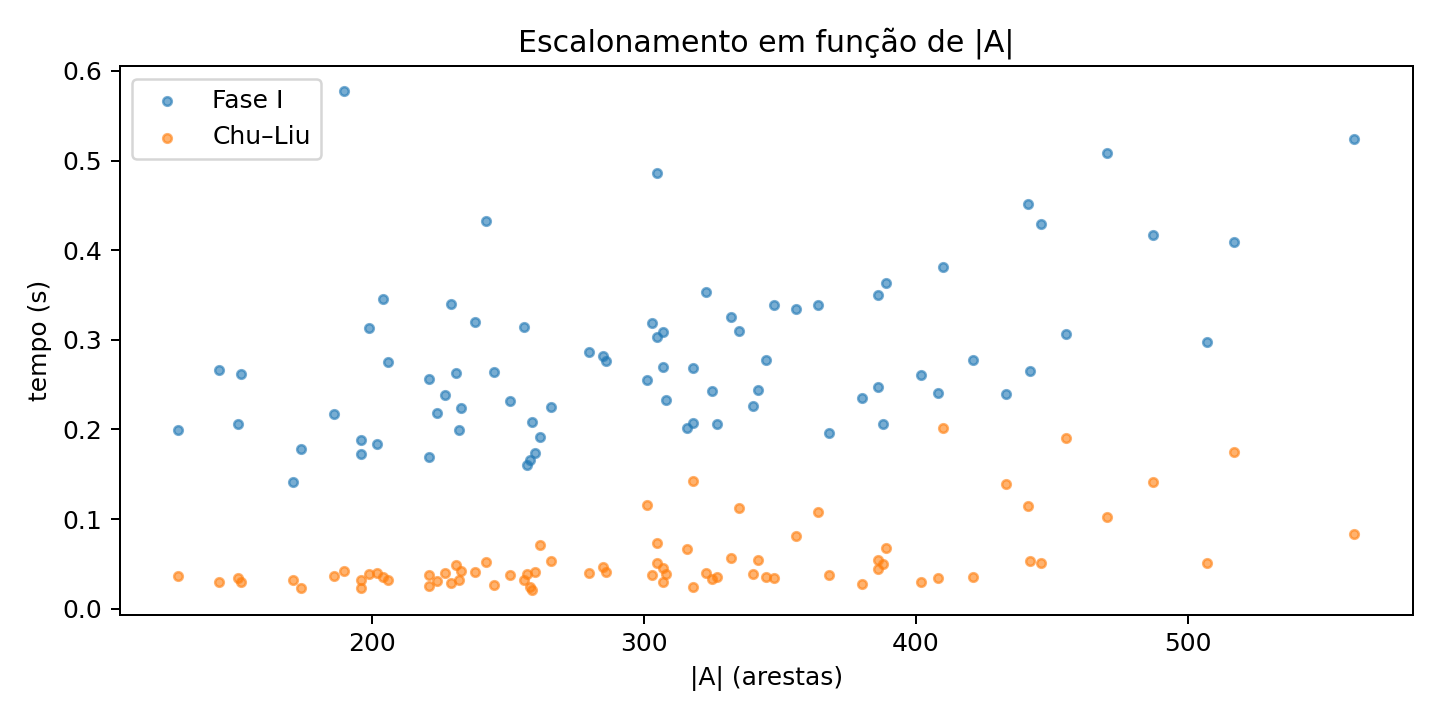
\includegraphics[width=.85\linewidth]{figures/fig_time_vs_edges_scatter.png}
    \caption{Escalonamento temporal em função de \(|A|\): comparação entre \emph{Chu--Liu} e Fase~I.}
    \label{fig:time-vs-edges}
\end{figure}

\begin{figure}[H]
    \centering
    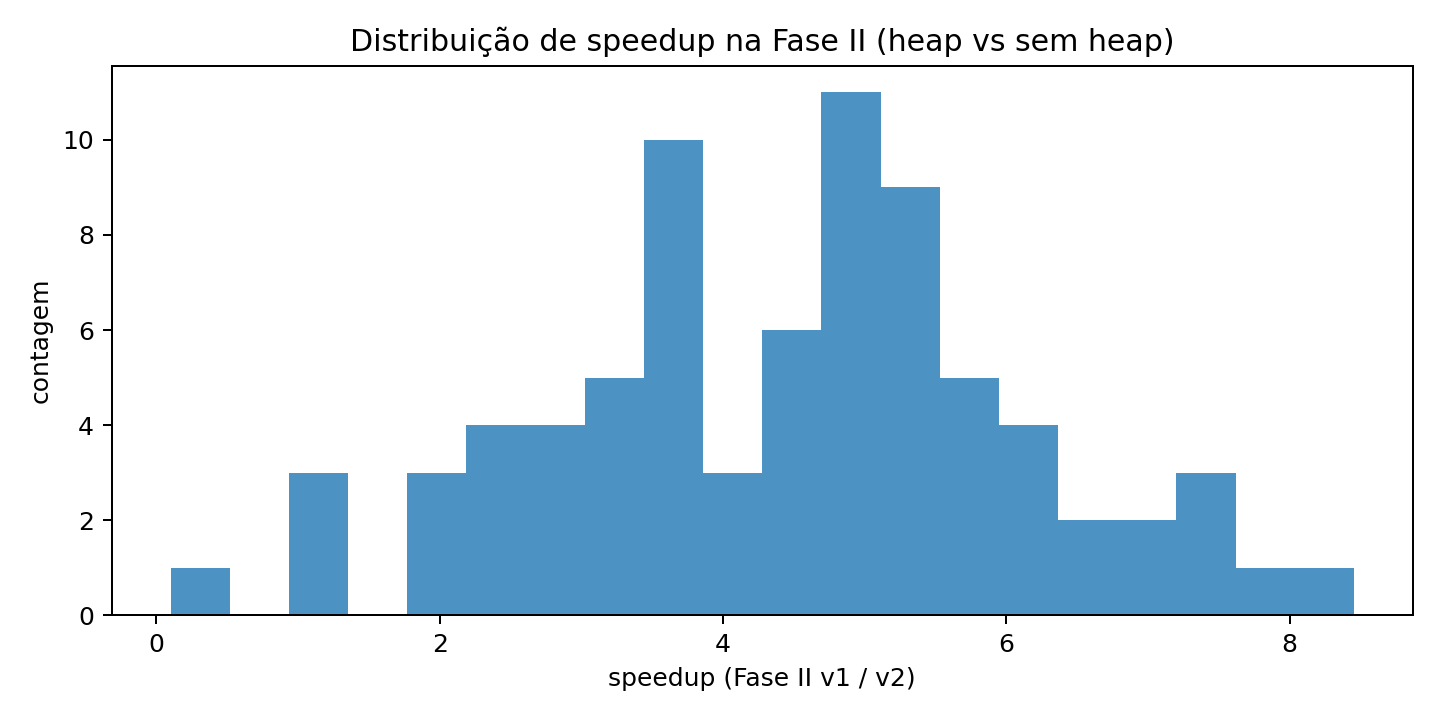
\includegraphics[width=.75\linewidth]{figures/fig_speedup_hist.png}
    \caption{Histograma de speedup na Fase~II (\(\text{v1}/\text{v2}\)): valores maiores que 1 indicam v2 (heap) mais rápida.}
    \label{fig:speedup}
\end{figure}

\begin{figure}[H]
    \centering
    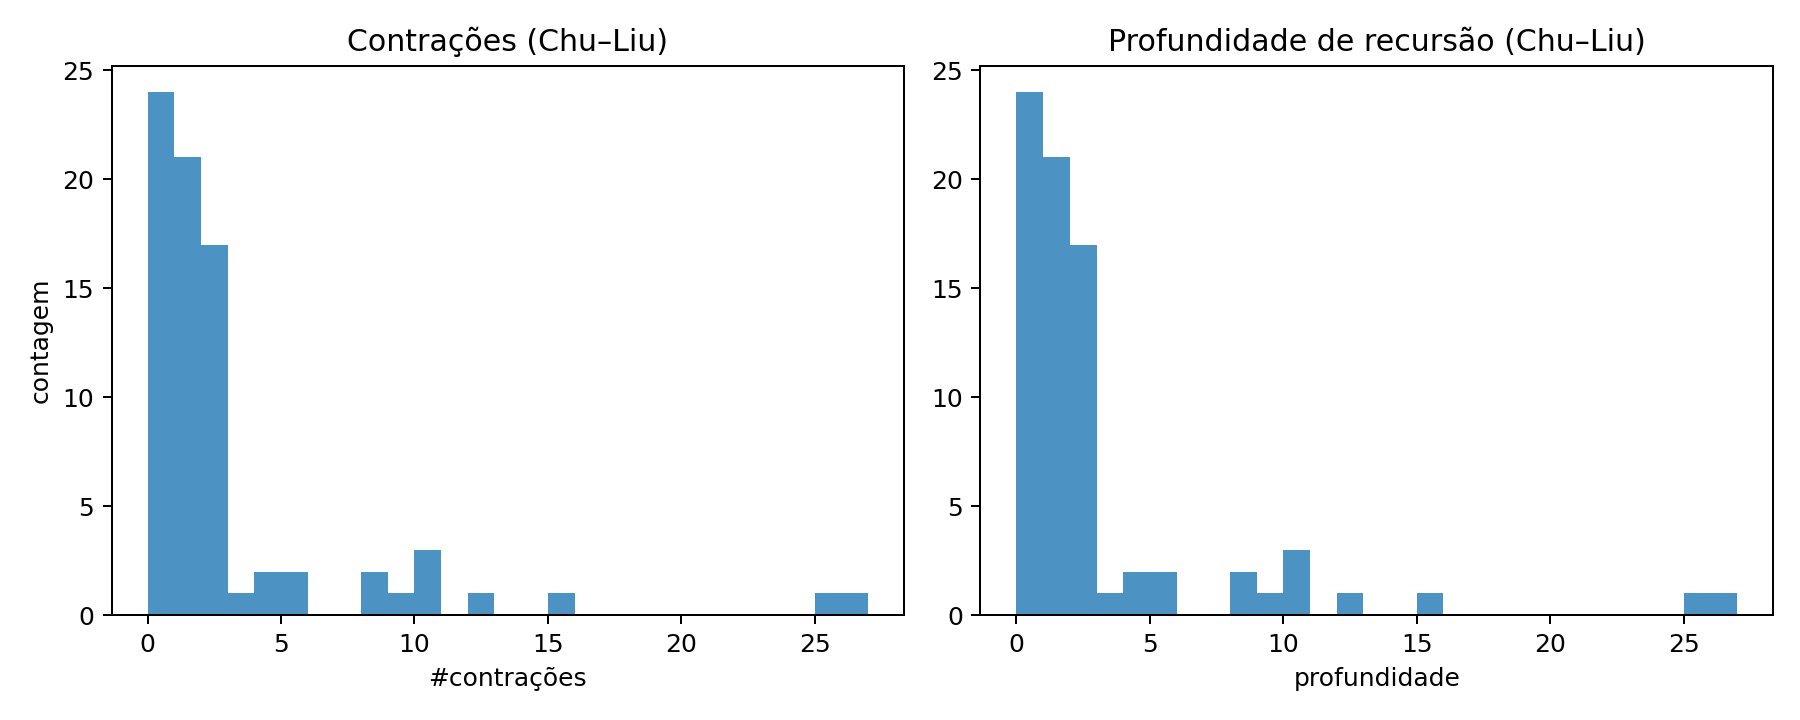
\includegraphics[width=.48\linewidth]{figures/fig_contractions_depth.png}
    \caption{Distribuições do número de contrações e da profundidade de recursão em \emph{Chu--Liu}.}
    \label{fig:contr-depth}
\end{figure}

\begin{figure}[H]
    \centering
    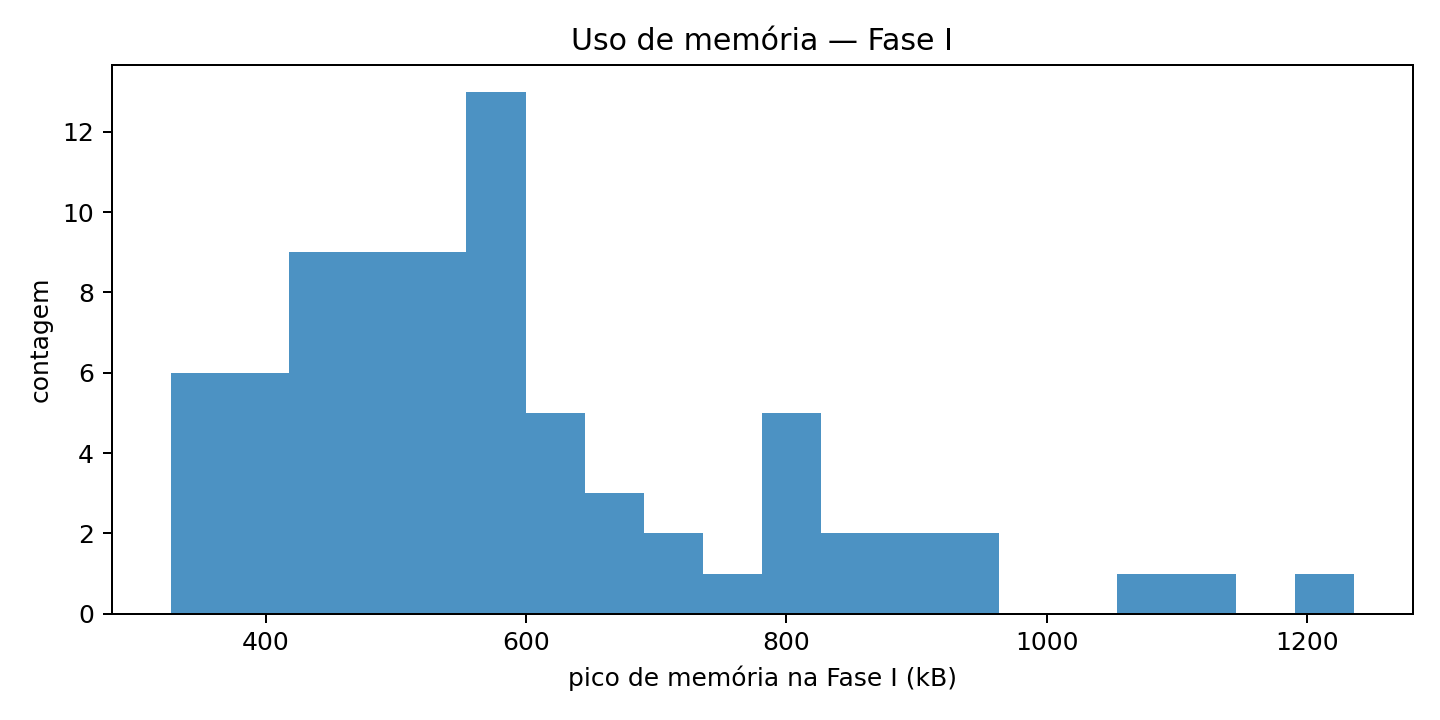
\includegraphics[width=.75\linewidth]{figures/fig_peakmem_hist.png}
    \caption{Pico de memória observado na Fase~I (kB).}
    \label{fig:peakmem}
\end{figure}

\begin{figure}[H]
    \centering
    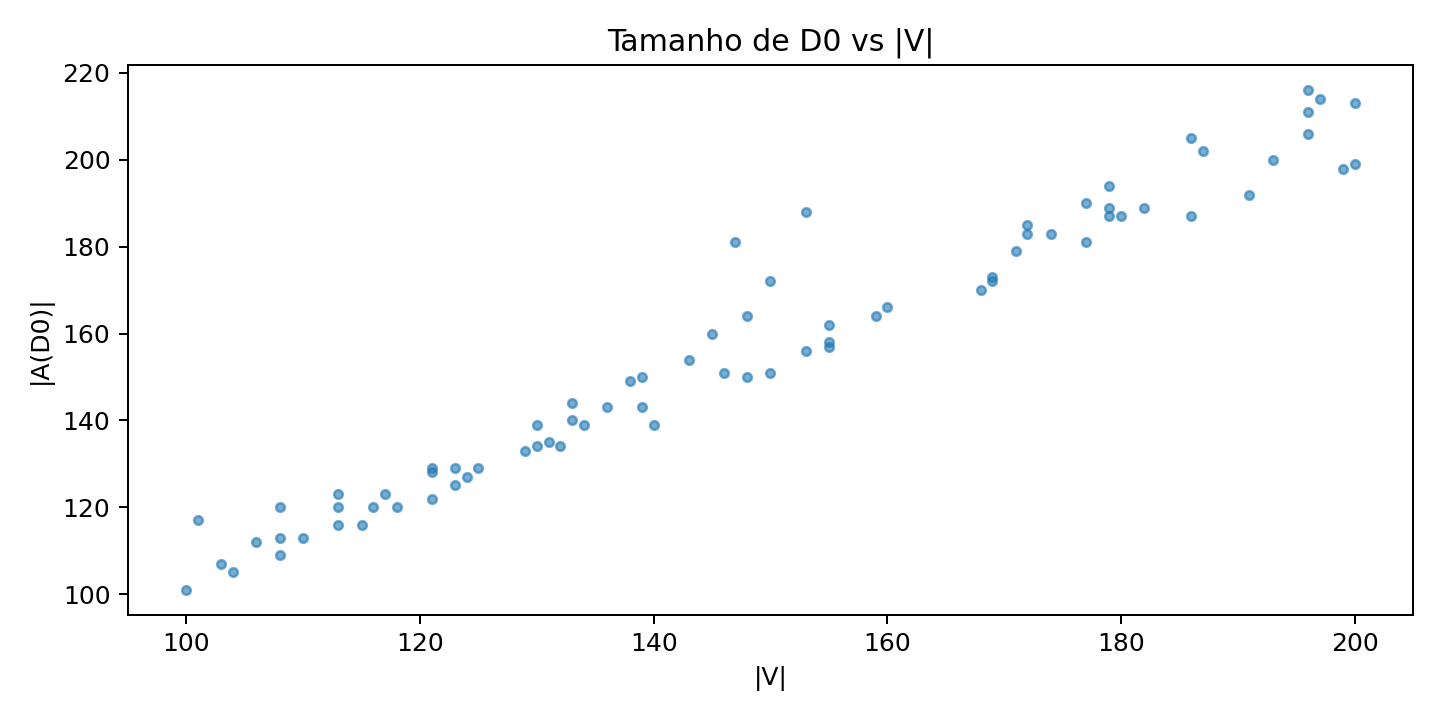
\includegraphics[width=.75\linewidth]{figures/fig_d0_edges_vs_vertices.png}
    \caption{Tamanho de \(D_0\) (número de arestas de custo reduzido zero) em função de \(|V|\).}
    \label{fig:d0-vs-v}
\end{figure}

Em síntese, os resultados empíricos alinham-se às previsões teóricas: custos coincidem e satisfazem complementaridade; o \emph{Chu--Liu} apresenta boa escalabilidade nas faixas testadas; a Fase~I de Frank tende a dominar o tempo; e a variação com heap reduz significativamente o custo da Fase~II, refletindo o uso de extrações \(\log n\). Essas observações reforçam o quadro de \cite{frank2014,schrijver2003comb}: a organização primal--dual de Frank torna explícitas as estruturas (cortes ativos, apertude) que explicam tanto a corretude quanto caminhos de otimização.


Os testes e as análises apresentados oferecem uma base robusta para a compreensão prática e teórica dos algoritmos de arborescência de custo mínimo, explicitando suas forças e nuances. Compreender os algoritmos teoricamente e validá-los empiricamente, porém, é apenas parte do desafio: como transformar esse conhecimento em aprendizagem efetiva para estudantes e profissionais?


A resposta que propomos envolve tornar essa experiência concreta e interativa. Para isso, desenvolvemos uma aplicação \textit{web} que permite acompanhar, passo a passo, o funcionamento de ambos os algoritmos, evidenciando suas semelhanças e diferenças de forma visual e manipulável.


A aprendizagem visual é especialmente útil nesse contexto: observar os algoritmos em ação, ver como normalizações transformam custos, como ciclos são contraídos e expandidos, e como potenciais duais guiam a seleção de arestas ajuda a fixar os conceitos apresentados de maneira que a leitura passiva não consegue. Antes de apresentar a aplicação em si, discutimos os fundamentos didáticos que orientaram seu design, explorando aspectos da didática de conceitos abstratos e princípios de interação humano-computador.
